\section{Variables Aleatòries Discretes}

\subsection{Definicions i conceptes relacionats. Funció generadora de probabilitat}

Sigui $(\Omega, \mathcal{A}, p)$ un espai de probabilitat i $X$ una variable aleatòria.

\begin{defi}
  $X$ és una \textbf{variable aleatòria discreta} si $Im(X)$ és numerable. \\
  Si $X$ és una variable aleatòria discreta, $Im(X) = \setb{x_{i}}_{i \geq 1}$. \\ 
  $X$ ve completament determinada pels valors $p(X=x_{i}) = p_{i}$.
\end{defi}

\begin{defi}
  Anomenem \textbf{funció de distribució} de X a:
  \[
    F_{X}(x)=p(X \leq x) = \sum_{x_{i}\leq x}p_{i}
  \]
\end{defi}

\begin{defi}
  Sigui $A \in \mathcal{B}$, la \textbf{mesura de probabilitat induïda sobre} $\real$ és:
  \[
    p_{X}(A) = \sum_{\substack{x_{i} \in A \\ x_{i}\in Im(X)}}p_{i}
  \]
  En particular, si $Im(X)\cap A = \varnothing$ aleshores $p_{X}(A) = 0 \implies$ obtenim una probabilitat puntual 
  (hi ha punts de $\real$ amb probabilitat $> 0$, a diferència de la mesura de Lebesgue).
\end{defi}

\begin{defi}
  Definim l'\textbf{esperança matemàtica} com: 
  \[
    \E [X] = \int_{\Omega}Xdp \underset{\text{def. de }\int_{\Omega}}{=\joinrel=\joinrel=\joinrel=\joinrel=} 
    \sum_{i\geq 1}x_{i}\cdot p(X=x_{i}) = \sum_{i\geq 1}x_{i}\cdot p_{i}
  \]
  Més en general, si $g(x)$ és una funció mesurable, 
  \[
    \E [g(X)] = \sum_{i\geq 1}g(x_{i})\cdot p(X=x_{i})
  \]
  En particular, 
  \[
    \E[X^{k}]=\sum_{i\geq 1}x_{i}^{k}\cdot p_{i}
  \]
  \[
    \V ar[X] = \E[X^{2}]-\E[X]^{2}=\sum_{i\geq 1}x_{i}^{2}\cdot p_{i} - \Big(\sum_{i\geq 1}x_{i}\cdot p_{i} \Big)^{2}
  \]
\end{defi}

\begin{defi}
  Prenem $X$, $Y$ variables aleatòries discretes amb $Im(X), \, Im(Y)$ numerables. \\
  El \textbf{vector de variables aleatòries} $(X,Y)$ ve completament caracteritzat per: 
  \[
    p_{(X,Y)}(x_{i},y_{j}) = p(X=x_{i}, Y=y_{j}) \qquad (x_{i}\in Im(X); y_{i}\in Im(Y))
  \]
\end{defi}

\newpage
Aleshores, tenim les següents propietats: \\\\
(i) $X$ i $Y$ són independents $\iff \forall x_{i}\in Im(X), \, \forall y_{j}\in Im(Y), 
\, p_{(X, Y)}(x_{i},y_{j}) = p_{X}(x_{i})\cdot p_{Y}(y_{j})$ \\\\
(ii) Si $X, \, Y$ són independents, $\E[X\cdot Y] = \E[X]\cdot \E[Y]$ \\\\

Sigui $X$ una variable aleatòria discreta amb $Im(X)\subseteq \n_{\geq0}$. En aquesta situació, 
tenim la següent definició:

\begin{defi}
  La \textbf{funció generadora de probabilitat associada a $X$} és: 
  \[
    G_{X}(z) = \sum_{i\geq 0}p(X=i)\cdot z^{i} = \sum_{i\geq 0}p_{i}\cdot z^{i}
  \]
  
  Una funció generadora de probabilitat és un objecte formal. En particular, $G_{X}(z)=\E[z^{X}]$.
\end{defi}

Si ens mirem les funcions generadores de probabilitat com funcions (en $\cx$), aleshores compleixen el següent:

\begin{prop}
  \begin{enumerate}
      \item []
      \item $G_{X}(0) = p(X=0)$
      \item $G_{X}(1) = 1$. A més, si $\abs{z}\leq 1 \, (z\in \cx) \implies \abs{G_{X}(z)}\leq 1$ \\
      Per tant, $G_{X}(z)$ (com a sèrie de potències) té radi de convergència $\geq 1$.
      \item $\E[X] = \dfrac{d}{dz}G_{X}(z)_{\big|z=1}$
      \item Més en general, $\E[(X)_{k}] = \dfrac{d^{k}}{dz^{k}}G_{X}(z)_{\big|z=1}$ \\
      En particular, $\V ar[X] = G_{X}''(1) + G_{X}'(1) - (G_{X}'(1))^{2}$
      \item Si $z\in \real, \, z \in [0,1]$, aleshores $G_{X}(z)$ és una funció creixent.
  \end{enumerate}
\end{prop}

La propietat fonamental de les funcions generadores de probabilitat és que permeten estudiar 
fàcilment sumes de variables aleatòries independents.

\begin{prop}
  Siguin $X, Y$ variables aleatòries discretes independents amb imatge en $\n$, i amb funcions 
  generadores de probabilitat $G_{X}(z), \, G_{Y}(z)$. Aleshores: 
  \[
    G_{X+Y}(z) = G_{X}(z)\cdot G_{Y}(z)
  \]
\end{prop}

\begin{col}
  Si $X_{1}, \ldots, X_{N}$ són variables aleatòries discretes independents amb imatge en $\n$, aleshores: 
  \[
    G_{X_{1}+\ldots+X_{N}}(z) = \prod_{i=1}^{N} G_{X_{i}}(z)
  \]
\end{col}

\subsection{Models de variables aleatòries discretes}

Seguidament veurem famílies importants de variables aleatòries discretes: \\

1) \underline{Variable aleatòria Bernoulli}: $X\sim B(p)$ \quad (un sol paràmetre) \\
Modela el llançament d'una moneda amb probabilitat d'èxit igual a p: 
\[
  p(X=1) = p, \quad p(X=0) = 1-p
\]
\begin{itemize}
    \item $G_{X}(z) = p\cdot z + (1-p)$ \quad (és una funció entera)
    \item $\E[X] = p$
    \item $\V ar[X] = p\cdot(1-p)$
\end{itemize}

\vspace{0.5cm}

2) \underline{Binomial}: $X\sim Bin(p,n)$ (o bé $B(p,n)$) \\
Nombre d'èxits al tirar una moneda $n$ vegades. L'èxit individual té probabilitat $p$, i cada 
tirada de la moneda és independent de la resta. 
\[
  \implies X=Y_{1}+\ldots+Y_{n} \text{ on } Y_{i}\sim B(p)
\]
\[
  p(X=i) = \binom{n}{i}\cdot p^{i}\cdot (1-p)^{n-i} \qquad i = 0,\ldots,n
\]
\begin{itemize}
    \item $G_{X}(z) = (p\cdot z + (1-p))^{n}$ \quad (és una funció entera)
    \item $\E[X] = n\cdot p$
    \item $\V ar[X] = n\cdot p\cdot (1-p)$
\end{itemize}

\vspace{0.5cm}

3) \underline{Poisson}: $X \sim Po(\lambda)$
\[
  p(X=k) = \frac{1}{k!}\cdot \lambda^{k}\cdot e^{-\lambda} \quad (k\in \n_{\geq 0})
\]
\begin{itemize}
    \item $G_{X}(z) = e^{\lambda(z-1)}$ \quad (és una funció entera)
    \item $\E[X] = \lambda$
    \item $\V ar[X] = \lambda$
\end{itemize}

\vspace{0.5cm}

4) \underline{Uniforme}: $X\sim U(N)$ \quad (on $Im(X) = \setb{1,2,\ldots, N}$) \\
\[
  p(X=k) = \frac{1}{n}
\]
\begin{itemize}
    \item $G_{X} = \dfrac{1}{N}\cdot \dfrac{1-z^{N}}{1-z}\cdot z$ \quad (sing. evitable en z = 1)
    \item $\E[X]=\dfrac{N+1}{2}$
    \item $\V ar[X] = \dfrac{N^{2}-1}{12}$
\end{itemize}

\newpage

5) \underline{Geomètrica}: $X\sim Geom(p) \quad \big(p\in(0,1)\big)$ \\
Nombre de tirades d'una moneda (amb probabilitat d'èxit $= p$) fins aconseguir el primer èxit.
\[
  p(X=k) = (1-p)^{k-1}\cdot p \qquad k = 1,2,\ldots
\]
\begin{itemize}
    \item $G_{X}(z) = \dfrac{p\cdot z}{1-(1-p)\cdot z}$ \quad (té un pol en $z=\dfrac{1}{1-p}$)
    \item $\E[X] = \dfrac{1}{p}$
    \item $\V ar[X] = \dfrac{1-p}{p^{2}}$
\end{itemize}

\vspace{0.5cm}

6) \underline{Binomial negativa}: $X\sim BinN(r, p)$ \\
Variable aleatòria que compta el nombre de tirades necessàries per aconseguir $r$ èxits. $\left(Im(X)=\setb{r,r+1,r+2, \ldots}\right)$
\[
  p(X=k) = \binom{k-1}{r-1}\cdot p^{r}\cdot(1-p)^{k-r}
\]
Podem interpretar una binomial negativa com una suma de geomètriques independents.
\begin{itemize}
    \item $G_{X}(z) = \left( \dfrac{p\cdot z}{1-(1-p)\cdot z} \right)^{r}$
    \item $\E[X] = \dfrac{r}{p}$
    \item $\V ar[X] = r\cdot \dfrac{1-p}{p^2}$
\end{itemize}

\newpage

\subsection{Distribucions condicionades i esperança condicionada}
Siguin $X,Y$ dues variables aleatòries discretes. Volem definir la noció de condicionar una 
variable aleatòria a l'altra (`` $Y\mid X$ '').

\begin{defi}
  Donat $x$ amb $p(X=x)>0$, diem que la \textbf{funció de probabilitat condicionada} de $Y$ amb $X$ és, per aquest valor de $x$:
  \[
    p_{Y\mid X}(y,x) = p(Y=y\mid X=x)
  \]
\end{defi}

\begin{defi}
  Amb les mateixes condicions que abans, la \textbf{funció de distribució de probabilitat condicionada} és:
  \[
    F_{Y\mid X}(y,x) = p(Y\leq y \mid X \leq x)
  \]
\end{defi}

\begin{obs}
  Si $X$ i $Y$ són independents, $X\mid Y=y \sim X$
\end{obs}

\begin{defi}
  L'\textbf{esperança condicionada} de $Y$ a $X=x$ és: 
  \[
    \psi(x) = \E[Y\mid X=x] = \sum_{y\in Im(Y)}(y\cdot p_{Y\mid X})(y,x)
  \]
  Amb aquesta definició estem definint una variable aleatòria $E[Y\mid X]$ que pren el valor 
  $\psi(x)$ amb probabilitat $p(X=x)$.
\end{defi}

\begin{prop}
  $\E\big[\E[Y\mid X]\big] = \E[Y]$
\end{prop}

\begin{obs}
  $\E[Y] = \sum\limits_{x\in Im(X)}\E[Y\mid X=x]\cdot p(X=x)$
\end{obs}

\begin{obs}
  $\E[Y\mid X]$ és la millor aproximació de $Y$ com a funció de X.
\end{obs}

\subsection{Suma de variables aleatòries discretes (Aplicació 1)}
Ja hem vist que si $X$ i $Y$ són variables aleatòries discretes amb imatge en $\n$, aleshores 
si són independents, $G_{X+Y}(z) = G_{X}(z)\cdot G_{Y}(z)$ \\
Si fem $Z=X+Y$: 
\[
  G_{Z}(z) = \sum_{n\geq0}p(Z=n)\cdot z^{n} = \sum_{r\geq0}p(X=r)\cdot z^{r} \cdot \sum_{s\geq0}p(Y=s)\cdot z^{s}
\]
\[
  \implies p(Z=n) = \sum_{r+s=n}p(X=r)\cdot p(Y=s) = \underbrace{\sum_{m=0}^{n}p(X=m)\cdot p(Y=n-m)}_{Convoluci\acute o}
\]
Aplicant aquest principi de l'ús de funcions generadores, tenim que: \\
\begin{enumerate}
    \item $X_{1}, X_{2}, \ldots , X_{n} \sim Ber(p)$ independents $\implies X_{1}+X_{2}+\ldots +X_{n} \sim Bin(n,p)$
    \item $X_{1}, X_{2}, \ldots , X_{n} \sim Geom(p)$ independents $\implies X_{1}+X_{2}+\ldots +X_{n} \sim BinN(n,p)$
    \item $X_{1}\sim Po(\lambda_{1}), \, X_{2}\sim Po(\lambda_{2}), \, X_{1}, X_{2}$ independents 
    \[
    \begin{rcases}
    G_{X_{1}}(z) = e^{-\lambda_{1}}\cdot e^{\lambda_{1}\cdot z} \\
    G_{X_{2}}(z) = e^{-\lambda_{2}}\cdot e^{\lambda_{2}\cdot z}
    \end{rcases}\implies G_{X_{1}+X_{2}}(z) = e^{-(\lambda_{1}+\lambda_{2})}\cdot e^{(\lambda_{1} + \lambda_{2})\cdot z}
    \]
    \[
      \hspace{-6cm}\implies X_{1} + X_{2} \sim Po(\lambda_{1} + \lambda_{2})
    \]
\end{enumerate}

\subsection{Arbres de Galton-Watson (Aplicació 2)}
Sigui $X$ una variable aleatòria discreta amb $Im(X)\subseteq \n_{\geq 0}$. \\
Considerem el següent procés estocàstic: \\
\begin{figure}[h]
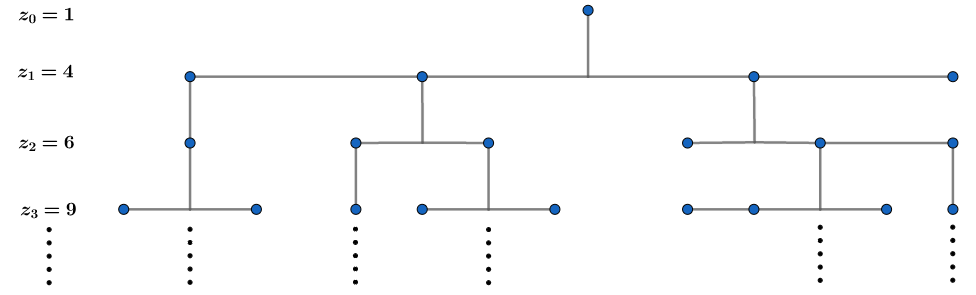
\includegraphics[scale=0.45]{G-WTree.png}
\caption*{\textbf{Arbre de Galton-Watson}}
\centering
\end{figure}
\\
$Z_{0} = 1$\\\\
En les següents generacions, el nombre de fills ve donat per la v.a. $X$.\\\\
$Z_{1} =$ nº de fills del primer individu (generació 0), seguint $X$.\\
$Z_{2} =$ nº de fills dels individus de la generació 1.\\
.\\
.\\
.\\
$Z_{n} =$ nº de descendents en la generació n-èssima.\\\\

\underline{Propietat fonamental}: el nombre de descendents d'un individu és independent del 
nombre de descendents de qualsevol altre individu. \\

\begin{lema}
  Sigui $N$ una variable aleatòria amb imatge en $\setb{1,2,3,\ldots}$.\\
  $X_{1},X_{2},X_{3},\ldots$ variables aleatòries independents (i independents amb $N$), amb 
  $X_{i}\sim X$. Prenem $Y=X_{1}+X_{2}+\ldots +X_{N}$\\
  $\implies G_{Y}(z)=G_{N}(G_{X}(z))$
\end{lema}

\begin{prop}
  $G_{Z_{n+m}}(z) = G_{Z_{n}}(G_{Z_{m}}(z))$. En particular $G_{Z_{n}}(z)=G_{X}\circ \overset{n)}{\ldots} \, \circ G_{X}(z)$
\end{prop}

\begin{obs}
  Podem calcular $\E[Z_{n}]$ i $\V ar[Z_{n}]$ a partir de la seva funció generadora de probabilitat:
  \[
    \E[Z_{n}] = \E[X]^{n}
  \]
  \[
    \V ar[Z_{n}] = 
    \begin{cases}
      n\cdot \V ar[X] \qquad &\text{si } \E[X] = 1 \\\\
      \dfrac{\V ar[X]\cdot (\E[X]^{n}-1)}{\E[X]-1} \quad &\text{si } \E[X]\not =1
    \end{cases}
  \]
\end{obs}

Ara, la pregunta que ens fem és: quan hi haurà extinció?\\
Si fem $A_{n} = \setb{Z_{n} = 0} \implies Extinci\acute o = \bigcup\limits_{n\geq1}A_{n}$\\
$\implies p(Extinci\acute o) = p(\bigcup\limits_{n\geq1}A_{n})$\\\\
$A_{1}\subseteq A_{2}\subseteq A_{3}\subseteq \ldots$\\\\
$
\begin{rcases}
  \text{Extingit a la primera gen}\implies \text{Extingit a la segona gen.} \implies \ldots \\
  \text{Extingit a la segona gen.}\centernot\implies \text{Extingit a la primera} \ldots
\end{rcases} \implies
$
\\\\
$\implies$ Tenim una successió creixent de successos.\\\\
$A_{1}\subseteq A_{2}\subseteq A_{3}\subseteq \ldots$ és creixent $\implies p(Extinci\acute o) = 
\lim\limits_{n\to\infty}p(A_{n}) = \lim\limits_{n\to\infty}p(Z_{n}=0)$\\

\begin{thm}[(Galton)]
  Si $\E[X] = \mu$; $p(X=0) \geq 0$\\
  I sigui $\alpha$ la solució més petita positiva de l'equació $G_{X}(z) = z$ (Aleshores $p(Extinci\acute o) = \alpha$)
  \begin{enumerate}
      \item Si $\mu < 1 \implies \alpha = 1$ \hspace{5.55cm} (\underline{règim subcrític})
      \item Si $\mu = 1 \implies \alpha = 1$ (sempre que $\V ar[X] \not = 0$) \hspace{1cm}(\underline{règim crític})
      \item Si $\mu > 1 \implies 0<\alpha<1$ \hspace{4.85cm} (\underline{règim supercrític})
  \end{enumerate}
\end{thm}
